\section{\textbf{Language Model Implementation}}

%%%%%%%%%%%%%%%%%%%%%%%%%%%%%%%%%%%%%%%%%%%%%%%%%%%%%%%%%%%%%%%%%%%%%%%%%%%%%%%%
\subsection{\textbf{Trigram Model}}

\subsubsection{\textbf{Symbols}}

\begin{itemize}
% \item We regard each sentence as a sequence $s$ of $n$ random variables, $X_1, X_2, \dots, X_n$. We have a special symbol $X_n=\text{STOP}$ to denote the end of this sentence.

\item For trigram language model, the second-order Markov assumption is made. The probability of any sequence 
$s=x_1\dots x_n$ is $P(X_1=x_1, X_2=x_2, \dots, X_n=x_n)=\Pi_{i=1}^{n} P\left(X_{i}=x_{i} | X_{i-2}=x_{i-2}, X_{i-1}=x_{i-1}\right)$.
% $$
% \begin{aligned}
% &P(X_1=x_1, X_2=x_2, \dots, X_n=x_n)=\\
% &\Pi_{i=1}^{n} P\left(X_{i}=x_{i} | X_{i-2}=x_{i-2}, X_{i-1}=x_{i-1}\right)
% \end{aligned}
% $$ 
We further assume that $x_{-1}=x_{0}=*$.

\item For any $i$ and any $x_{i-2}, x_{i-1}, x_{i}$ we have $P\left(X_{i}=x_{i} | X_{i-2}=x_{i-2}, X_{i-1}=x_{i-1}\right)=q\left(x_{i} | x_{i-2}, x_{i-1}\right)$.
% $$
% \begin{aligned}
% &P\left(X_{i}=x_{i} | X_{i-2}=x_{i-2}, X_{i-1}=x_{i-1}\right)\\
% &=q\left(x_{i} | x_{i-2}, x_{i-1}\right)
% \end{aligned}
% $$
Then the model takes the form $p\left(x_{1} \ldots x_{n}\right)=\prod_{i=1}^{n} q\left(x_{i} | x_{i-2}, x_{i-1}\right)$ for any sequence $s$.
\item For any trigram $(u, v, w)$, and a finite set $\mathcal{V}$, define the probability of the appearance of the word $w$ immediately after the bigram $(u,v)$ is $q(w|u,v)$, $w \in \mathcal{V} \cup\{S T O P\}$ and $u, v \in \mathcal{V} \cup\{*\}$.
\end{itemize}

\subsubsection{\textbf{Maximum-Likelihood Estimates}}

\hfill 

We use maximum-likelihood estimates to estimate $q\left(w | u, v\right)$. Define $c(u, v, w)$ to be the number of times that the trigram $(u, v, w)$ is seen in the training corpus. Similarly, define $c(u, v)$ to be the number of times that the bigram $(u, v)$ is seen in the corpus. Then for any $w, u, v$ we have $q(w | u, v)=\frac{c(u, v, w)}{c(u, v)}$.

\subsubsection{\textbf{Implementations}}

We implemented the following functions:

In Algorithm~\ref{fit_sentence}, for trigram model, we will only need to store bigram and trigram counts.

\begin{algorithm}[]
  \caption{$fit\_sentence$}
  \label{fit_sentence}
  \KwIn{$sentence$ as a List}
  \KwOut{None but update $self.unigram$, $self.bigram$ and $self.trigram$}
  Generate all the trigrams and bigrams and stored in Lists\;
  \For{each trigram $t$ in trigram List}
  {
    Update trigram appearance counter\;
  }
  \For{each bigram $b$ in bigram List}
  {
    Update bigram appearance counter\;
  }
\end{algorithm}


In Algorithm~\ref{norm}, we calculate the log-probability as 

$$
\begin{aligned}
\log q(w | u, v)&=\log\frac{c(u, v, w)}{c(u, v)}\\
&=\log c(u, v, w) - \log c(u, v)
\end{aligned}
$$

Given previous words, Algorithm~\ref{cond_logprob} return the log of the conditional probability of word. If the trigram $(u, v, w)$ is never seen, then we return the log of a very small number to represent the low probability.

\begin{algorithm}[]
  \caption{$norm$}
  \label{norm}
  \KwIn{$self.trigram$, $self.bigram$ and $self.unigram$ as dicts}
  \KwOut{$self.model$}
  \For{each trigram $t$ in $self.trigram$}
  {
    Find the corresponding bigram $b$\;
    $//$ Update the store $q(w|u,v)$
    $self.model = \log(self.trigram[t]) - \log(self.bigram[b])$  
  }
\end{algorithm}

\begin{algorithm}[]
  \caption{$cond\_logprob$}
  \label{cond_logprob}
  \KwIn{$self.model$, $word\ w$, $previous [u,v]$}
  \KwOut{the log-probability of $(u, v, w)$}
  \If{trigram $(u, v, w)$ in $self.model$}
  {
    return $self.model[(u, v, w)]$
  }
  \Else
  {
    $//$ Return the log of a very small number 
    return $self.lbackoff$
  }
\end{algorithm}




%%%%%%%%%%%%%%%%%%%%%%%%%%%%%%%%%%%%%%%%%%%%%%%%%%%%%%%%%%%%%%%%%%%%%%%%%%%%%%%%
\subsection{\textbf{Smoothing method}}

Add-$\delta$ smoothing is chosen to ensure my language model outputs a non-zero and valid probability distribution for OOV words.

Compared with Algorithm~\ref{fit_sentence}, when doing smoothing, we add the vocabulary size $\mathcal{V}$ in the denominator, so we need the number of distinct tokens. That's why we update the unigram counter in Algorithm~\ref{fit_sentence2}.

\begin{algorithm}[]
  \caption{$fit\_sentence$}
  \label{fit_sentence2}
  \KwIn{$sentence$ as a List}
  \KwOut{None but update $self.unigram$, $self.bigram$ and $self.trigram$}
  $//$ As above\;
  \For{each unigram $w$ in sentence List}
  {
    Update unigram appearance counter\;
  }
\end{algorithm}

In Algorithm~\ref{norm2}, after using Add-$\delta$ smoothing, we calculate the log-probability as 

$$
\begin{aligned}
&\log q(w | u, v)=\log\frac{c(u, v, w)+\delta}{c(u, v)+\delta * \mathcal{V}}\\
&=\log \Big(c(u, v, w)+\delta \Big) - \log \Big(c(u, v) + \delta * \mathcal{V} \Big)
\end{aligned}
$$

\begin{algorithm}[]
  \caption{$norm$}
  \label{norm2}
  \KwIn{$self.trigram$, $self.bigram$ and $self.unigram$ as dicts, $self.delta$ as smoothing parameter}
  \KwOut{$self.model$}
  \For{each trigram $t$ in $self.trigram$}
  {
    find the corresponding bigram $b$\;
    $//$ Update the store $q(w|u,v)$ using smoothing
    $self.model = \log(self.trigram[t]+self.delta) - \log(self.bigram[b]+self.delta*len(self.unigram.keys()))$
  }
\end{algorithm}

Given previous words, Algorithm~\ref{cond_logprob2} return the log of the conditional probability of word. Compared with Algorithm~\ref{cond_logprob}, if the trigram $(u, v, w)$ is never seen, we return

$$
\begin{aligned}
&\log q(w | u, v)=\log\frac{\delta}{c(u, v)+\delta * \mathcal{V}}\\
&=\log \Big(\delta \Big) - \log \Big(c(u, v) + \delta * \mathcal{V} \Big)
\end{aligned}
$$

\begin{algorithm}[]
  \caption{$cond\_logpro$}
  \label{cond_logprob2}
  \KwIn{$self.model$, $word\ w$, $previous (u,v)$ and $self.delta$}
  \KwOut{the log-probability of $(u, v, w)$}
  \If{trigram $(u, v, w)$ in $self.model$}
  {
    return $self.model[(u, v, w)]$
  }
  \Else
  {
    find the corresponding bigram $b$\;
    \If{bigram b in self.bigram}
    {
        return $\log(self.delta) - \log(self.bigram[b]+self.delta*len(self.unigram.keys()))$
    }
    \Else{
        return $-\log len(self.unigram.keys())$
    }
  }
\end{algorithm}

%%%%%%%%%%%%%%%%%%%%%%%%%%%%%%%%%%%%%%%%%%%%%%%%%%%%%%%%%%%%%%%%%%%%%%%%%%%%%%%%
\subsection{\textbf{Hyperparameter tuning and data used for tuning}}

The only hyperparameter needed to tune is $\delta$. So I tune the parameter $\delta$ on the dev set of the three corpus. The results are shown in the figure~\ref{fig:delta}.

\begin{figure}[h]
\caption{Perplexity-Delta Graph of dev set for different corpus}
\centering
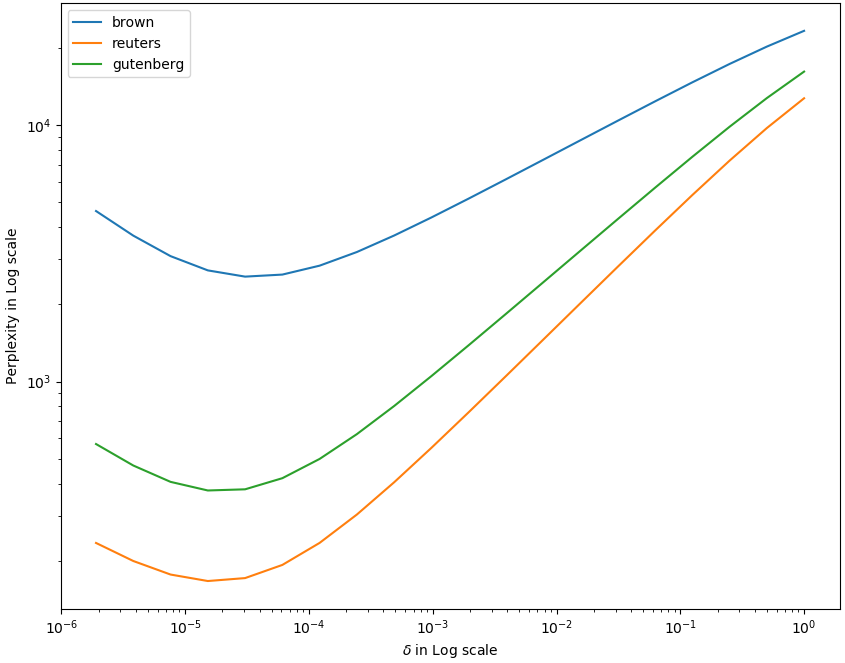
\includegraphics[width=0.45\textwidth]{files/figs/Perplexity-Delta.png}
\label{fig:delta}
\end{figure}

We let $\delta$ ranges between $1/2^{0}$ and $1/2^{20}$. Perplexity reaches the lowest point when $\delta$ equals $1/2^{15}$, which is $3.0517578125e-05$. So we choose to set $\delta$ as this value.

